\documentclass[12pt]{article}
\newcommand{\Version}{2.0.0} 
\newcommand{\ReleaseDate}{July 12th, 2021} 

\usepackage[letterpaper,margin=0.5in,bottom=0.75in]{geometry}
\usepackage{amsmath}
\usepackage{amssymb}
\usepackage{dsfont}
\usepackage{bbm}
\usepackage{stmaryrd}
\usepackage{graphicx}
\usepackage{pbox}
\usepackage{hyperref}
\usepackage{changepage}
\usepackage[dvipsnames,usenames]{color}

\setcounter{tocdepth}{4}
\setcounter{secnumdepth}{4}

\usepackage{caption}
\captionsetup{justification=raggedright,singlelinecheck=false}

\usepackage{tikz}
\usetikzlibrary{arrows,automata,arrows.meta}

\usepackage{mdframed}

\mdfdefinestyle{mystyle}{
    backgroundcolor=lightgray!10, 
    innertopmargin=5mm, 
    innerbottommargin=5mm, 
    innerleftmargin=5mm, 
    innerrightmargin=5mm 
}


\usepackage{bold-extra}
  
\hypersetup{
pdftitle={PhysiCell User Guide \Version}, 
pdfauthor={Paul Macklin and the PhysiCell Project}, 
pdfsubject={PhysiCell},
pdfproducer={http://MathCancer.org}, 
pdfkeywords={PhysiCell,agent-based model,simulation}, 
colorlinks=true,
linkcolor=blue, 
citecolor=red, 
filecolor=magenta,
urlcolor=blue
}

 
\usepackage[square,comma,numbers,sort&compress]{natbib}
\usepackage[nottoc]{tocbibind}

\newcommand{\braces}[1]{\left\{#1\right\}}
\newcommand{\abs}[1]{\left|#1\right|}
\renewcommand{\vec}[1]{\mathbf{#1}}
\newcommand{\mean}[1]{\langle #1 \rangle}
\newcommand{\norm}[1]{\left|\left|{#1}\right|\right|}

\newcommand{\beq}{\begin{equation}}
\newcommand{\eeq}{\end{equation}}
\newcommand{\beqa}{\begin{eqnarray}}
\newcommand{\eeqa}{\end{eqnarray}}
\newcommand{\beqaN}{\begin{eqnarray*}}
\newcommand{\eeqaN}{\end{eqnarray*}}

\newcommand{\micron}{\mu\textrm{m}}
\newcommand{\specialcell}[2][c]{%
  \begin{tabular}[#1]{@{}c@{}}#2\end{tabular}}

\newcommand{\boldrho}{\rho\hspace{-5.1pt}\rho}
% \newcommand{\grvec}[1]{#1\hspace{-6pt}#1\hspace{-6pt}#1\hspace{1pt}}
\newcommand{\grvec}[1]{\boldsymbol{#1}}
\newcommand{\one}{\mathds{1}}

\newcommand{\hp}{\circ}%{\odot}%{\circ}
\newcommand{\hd}{\hspace{-1.6mm}\fatslash}%{\oslash}'

\setlength{\parskip}{1em}
\setlength{\parindent}{0in}

\newcommand{\code}[1]{\verb|#1|}
\renewcommand{\v}{\verb}
\renewcommand{\t}[1]{\left[\mathrm{#1}\right]}
\renewcommand{\tt}[1]{{\small \left[\texttt{#1}\right] }}

\newcommand{\smallcode}[1]{\textbf{\texttt{#1}}} 
%\newcommand{\smallcode}[1]{\textbf{\v|#1|}} 

\newcommand{\red}[1]{\textcolor{red}{#1}}
\newcommand{\blue}[1]{\textcolor{blue}{#1}}
\newcommand{\magenta}[1]{\textcolor{magenta}{#1}}
\newcommand{\FIX}{}%{\textbf{\red{[FIX ME]}}}
\newcommand{\DONE}{}%{\textbf{\blue{[DONE]}}}
\newcommand{\FINISH}{}%{\magenta{[FINISH ME]}}

\newcommand{\TOClink}{\begin{center}\hrule\vskip-5pt\phantom{.}\hfill[Return to \hyperlink{TOC}{Table of Contents}.]\hfill\phantom{.}\vskip3pt\hrule\end{center}}
\begin{document}


\author{PhysiBoSS Project}
\title{PhysiBoSS User Guide (Version \Version)}
\date{Revision: \today}

\maketitle

\setlength{\parskip}{0in}
\hypertarget{TOC}{}
\tableofcontents
\setlength{\parskip}{8pt}

\section{Introduction and citing PhysiBoSS \DONE}
This user guide will teach you how to use PhysiBoSS \cite{letort2019physiboss, ponce2022physiboss}, as well as document the key classes and functions. Wherever possible, it will demonstrate with specific examples. Please note that this guide will be periodically updated. 

The original PhysiBoSS paper was published in PLoS Computational Biology \cite{letort2019physiboss}, and it's official inclusion as an addon on PhysiCell\cite{ref:PhysiCell} is on BioRxiv \cite{ponce2022physiboss}. \\
\\
If you use PhysiBoSS, please cite it as: \\
\\
\phantom{ }\hspace{.075\textwidth}\parbox[top]{0.85\textwidth}{%
We implemented and solved our model using PhysiBoSS (Version \Version) [1,2]. \\

[1] G. Letort, A. Montagud, G. Stoll, R. Heiland, E. Barillot, P. Macklin, A. Zinovyev, and L. Calzone.
Physiboss: a multi-scale agent-based modelling framework integrating physical dimension and cell
signalling. Bioinformatics, 35(7):1188–1196, 2019.


[2] M. Ponce-de Leon, A. Montagud, V. Noël, G. Pradas, A. Meert, E. Barillot, L. Calzone, and A. Valencia.
Physiboss 2.0: a sustainable integration of stochastic boolean and agent-based modelling frameworks.
bioRxiv, pages 2022–01, 2022.

}\\
\\

Because PhysiBoSS is an addon on PhysiCell, we suggest you also cite it:  

\phantom{ }\hspace{.075\textwidth}\parbox[top]{0.85\textwidth}{%
We implemented and solved the model using PhysiBoSS (Version \Version) [1,2], an addon of PhysiCell[3] \\

[1] G. Letort, A. Montagud, G. Stoll, R. Heiland, E. Barillot, P. Macklin, A. Zinovyev, and L. Calzone.
Physiboss: a multi-scale agent-based modelling framework integrating physical dimension and cell
signalling. Bioinformatics, 35(7):1188–1196, 2019.


[2] M. Ponce-de Leon, A. Montagud, V. Noël, G. Pradas, A. Meert, E. Barillot, L. Calzone, and A. Valencia.
Physiboss 2.0: a sustainable integration of stochastic boolean and agent-based modelling frameworks.
bioRxiv, pages 2022–01, 2022.

[3] A. Ghaffarizadeh, R. Heiland, S.H. Friedman, S.M. Mumenthaler, and P. Macklin. PhysiCell: an Open Source Physics-Based Cell Simulator for 3-D Multicellular Systems, PLoS Comput. Biol. 14(2): e1005991, 2018. DOI: \href{https://dx.doi.org/10.1371/journal.pcbi.1005991}{10.1371/journal.pcbi.1005991}.
\\
}

\TOClink

\section{Getting started: Your First Simulation}
\label{sec:getting_started}

PhysiBoSS comes with an easy to use example to quickly start simulating your first PhysiBoSS project. First, to load the project, run : 

\begin{verbatim}
   make physiboss-cell-lines-sample
\end{verbatim}

This will copy all the project files to the root, config and custom\_modules folder. Then, to build the project, run : 

\begin{verbatim}
   make
\end{verbatim}

Finally, to execute the project, run : 

\begin{verbatim}
   ./PhysiBoSS_Cell_Lines
\end{verbatim}


\TOClink

\section{PhysiBoSS XML definition}
\label{sec:physiboss_xml_definitions}

Here is an example of the XML configuration of a PhysiBoSS model : 
\begin{verbatim}
   <cell_definition name="..." ID="...">
      ...
      <phenotype>
         ...
         <intracellular type="maboss">
            <bnd_filename>./config/model_0.bnd</bnd_filename>
            <cfg_filename>./config/model.cfg</cfg_filename>
            <time_step>10</time_step>
            <scaling>60</scaling>
            <time_stochasticity>0.0</time_stochasticity>
            <initial_values>
               <initial_value node="A">1</initial_value>
               <initial_value node="C">0</initial_value>
            </initial_values>
            <mutations>
               <mutation node="C">0.0</mutation>
            </mutations>
            <parameters>
               <parameter name="$time_scale">0.2</parameter>
            </parameters>	
         </intracellular>
         ...
      </phenotype>
      ...
   </cell_definition>
\end{verbatim}

This example use all available options of PhysiBoSS \Version. Let's look at them one by one : 

\begin{verbatim}
   <bnd_filename>./config/model_0.bnd</bnd_filename>
   <cfg_filename>./config/model.cfg</cfg_filename>
\end{verbatim}

A MaBoSS model is defined by two files : one for the model definition (BND file) and one for the simulation settings (CFG file). Here we configure the MaBoSS model which will be used in the PhysiBoSS simulation. 

\begin{verbatim}
   <time_step>10</time_step>
\end{verbatim}

PhysiCell will update its internal mechanisms regularly, depending on the time scale of the process described: diffusion of molecules in the environment will be governed by a short time scale, so its update will have to be performed very often (usually every seconds), while cell cycle progression will be governed by a large time scale so its update will be performed less frequently (usually every few minutes). A similar mechanism is used for PhysiBoSS, where the status of the MaBoSS model will be updated at every time\_step. Since this is model-dependent, we leave it to the user to define the appropriate time\_step.

\begin{verbatim}
   <scaling>60</scaling>
\end{verbatim}
Now let us suppose that our PhysiBoSS model is updating every 10 minutes, meaning that every 10 minutes, we will update the inputs of the MaBoSS model, simulate it, and the obtain its outputs nodes (phenotypes). The follow up question is how long should we simulate our MaBoSS model. A MaBoSS model has its own time unit since it contains kinetic rates for (in)activation, which is not always the same as PhysiCell unit (usually minutes) and we might have to adapt the simulation duration to PhysiCell unit. This is done using the scaling parameter. Let us suppose that the MaBoSS model's unit is hours. Then we need to set our scaling parameter to 60 so that every 10 minutes, PhysiBoSS will run the MaBoSS model for time\_step / scaling = 10/60 = 1/6 hours. Another way to see this scaling parameter is that if you want to run you MaBoSS simulation for 20 (MaBoSS time unit), you need to set scaling = time\_step / maboss\_simulation\_time.  

\begin{verbatim}
   <time_stochasticity>0.0</time_stochasticity>
\end{verbatim}
Biology is governed by many stochastic processes, and thus there is always noise in the duration of its processes. This is observed by the loss of synchronization of cell populations, for example is study about cell cycle progression. Cells at the beginning of the experiment can show synchronized cell cycle progression, but after a few cycles this synchronization will be lost. In PhysiBoSS, while we still have an heterogenous response of our MaBoSS models, when we select a large enough time\_step we can end up in a situation where all our cells are synchronized (by the update at regular time\_step). In order to avoid this artificial synchronization, we introduce a parameter called time\_stochasticity that will modify the value of the time\_step for every cell, so that it follows a Log Normal distribution with an average equal to time\_step, with a deviation a exp(time\_stochasticity). This allows cells to naturally lose their artificial synchronicity.

\begin{verbatim}
   <initial_values>
      <initial_value node="A">1</initial_value>
      <initial_value node="C">0</initial_value>
   </initial_values>
\end{verbatim}

While the initial values are defined by default in the model CFG file, we provide the possibility for the user to modify them in the XML configuration. The value can be any real number in [0,1].

\begin{verbatim}
   <mutations>
      <mutation node="C">0.0</mutation>
   </mutations>
\end{verbatim}
We also provide the possibility of applying mutations in the XML definition. For now, the value can only be 0 or 1, but we are planning to include gradual mutations in future releases. 

\begin{verbatim}
   <parameters>
      <parameter name="$time_scale">0.2</parameter>
   </parameters>
\end{verbatim}
Finally, we are also providing the possibility of modify parameter values directly in the XML definition. 
\TOClink

\section{PhysiBoSS API : MaBoSSIntracellular class}
\label{sec:physiboss_api}
%\begin{verbatim}
%	void start()
%\end{verbatim}
%This methods initialize the intracellular model. 
%

Here we expose the functions which are available in the MaBoSSIntracellular class, to query and control the state of the PhysiBoSS model. This is usually done in the custom code, for example in a custom implementation of update\_phenotype. Here is a simple example of such an implementation : 

\begin{verbatim}
void custom_update_phenotype( Cell* pCell, Phenotype& phenotype, double dt )
{
   // Checks if it is time to update the intracellular model
   if (pCell->phenotype.intracellular->need_update())
   {
      // Query the index of the density "Ainhib"
      static int ainhib_index = microenvironment.find_density_index( "Ainhib" );
      
      // Query the threshold from the user parameters to activate the node anti_A
      static double ainhib_threshold = parameters.doubles("ainhib_threshold");
	
      // Query the concentration of the internalized substrate Ainhib
      double ainhib_cell_concentration = 
         pCell->phenotype.molecular.internalized_total_substrates[ainhib_index];
      
      // Activates the node anti_A if the concrentration of the internalized substrate 
      // Ainhib is above the defined threshold
      pCell->phenotype.intracellular->set_boolean_variable_value(
         "anti_A", 
         ainhib_cell_concentration >= ainhib_threshold
      );
		
      // Run the MaBoSS simulation
      pCell->phenotype.intracellular->update();
	
      // We define the prosurvival phenotype accoding to the boolean value of the 
      // PhysiBoSS node C
      double prosurvival_value =
         pCell->phenotype.intracellular->get_boolean_variable_value("C") ? 1.0 : 0.0;
	
      // We query the indexes of the start and end phases of the live cell cycle model
      static int start_phase_index = phenotype.cycle.model().find_phase_index(
         PhysiCell_constants::live 
      ); 
      static int end_phase_index = phenotype.cycle.model().find_phase_index(
         PhysiCell_constants::live 
      );
      
      // We defined a new value for the cell cycle transition, based on the
      // prosurvival phenotype
      double multiplier = ( ( prosurvival_value * 20 ) + 1 ); 
      
      phenotype.cycle.data.transition_rate(start_phase_index,end_phase_index) =
         multiplier 
         * phenotype.cycle.data.transition_rate(start_phase_index,end_phase_index
      );
   }	
}

\end{verbatim}

This example will activate the input node anti\_A of the PhysiBoSS model if the internalized concentration of the sbstrate Ainhib is above the threshold defined in the user parameters. It will then run the MaBoSS simulation, and will modify the cell cycle transition rate according to the prosurvival phenotype defined by the node C. 

Now let us look at the methods available in the PhysiBoSS API : 

\begin{verbatim}
   void update()
\end{verbatim}
This method update the intracellular model : it runs the MaBoSS simulation for the defined time\_step. 

\begin{verbatim}
   bool need_update()
\end{verbatim}
This method checks if it is time to update the intracellular model, i.e. if the last simulation occurred more than a time\_step ago. 

\begin{verbatim}	
   bool has_variable(std::string name)
\end{verbatim}
This method checks if a variable exists in the intracellular model.

\begin{verbatim}	
   bool get_boolean_variable_value(std::string name)
\end{verbatim}
This method returns the boolean value of a given variable in the intracellular model.

\begin{verbatim}	
   void set_boolean_variable_value(std::string name, bool value)
\end{verbatim}
This method set the boolean value of a given variable in the intracellular model.

\begin{verbatim}
   double get_parameter_value(std::string name)
\end{verbatim}
This methods returns the value of a parameter of the intracellular model.

\begin{verbatim}	
   void set_parameter_value(std::string name, double value)
\end{verbatim}
This method set the value of a given parameter of the intracellular model.

\begin{verbatim}	
   std::string get_state()
\end{verbatim}
This method returns a string with the current state of the intracellular model.

\begin{verbatim}	
   void print_current_nodes()
\end{verbatim}
This method prints the current state of the intracellular model to the standard output.


\TOClink


\section{PhysiBoSS Makefile}
\label{sec:physiboss_makefile}

The first part of the Makefile specific to PhysiBoSS is an header to setup the path of the include and library directories : 

\begin{verbatim}
ifndef MABOSS_MAX_NODES
   MABOSS_MAX_NODES = 64
endif

MABOSS_DIR = addons/PhysiBoSS/MaBoSS-env-2.0/engine
CUR_DIR = $(shell pwd)

ifneq ($(OS), Windows_NT)
   LDL_FLAG = -ldl
endif

LIB := -L$(CUR_DIR)/$(MABOSS_DIR)/lib -lMaBoSS-static $(LDL_FLAG)
INC := -DADDON_PHYSIBOSS -I$(CUR_DIR)/$(MABOSS_DIR)/include -DMAXNODES=$(MABOSS_MAX_NODES)

ifeq ($(shell expr $(MABOSS_MAX_NODES) '>' 64), 1)
  LIB := -L$(CUR_DIR)/$(MABOSS_DIR)/lib -lMaBoSS_$(MABOSS_MAX_NODES)n-static $(LDL_FLAG)
endif
\end{verbatim}
Here the only part that a user should modify is the value of the default MABOSS\_MAX\_NODES, according to the MaBoSS model size, to choose which version of libMaBoSS will be used. We provide libMaBoSS libraries for up to 64 nodes (default), 128 nodes, 256 nodes and 512 nodes. 
 
\begin{verbatim}
PhysiBoSS_OBJECTS := maboss_network.o maboss_intracellular.o
...
ALL_OBJECTS := $(PhysiCell_OBJECTS) $(PhysiCell_custom_module_OBJECTS) $(PhysiBoSS_OBJECTS)
...
all: MaBoSS main.cpp $(ALL_OBJECTS)
   $(COMPILE_COMMAND) $(INC)  -o $(PROGRAM_NAME) $(ALL_OBJECTS) main.cpp $(LIB)
\end{verbatim}

Then, we need to defined the PhysiBoSS\_OBJECTS, and add them to the ALL\_OBJECTS variable. Finally, we need to add MaBoSS to the all directive, to ensure that it will be installed if needed. 

\begin{verbatim}
...
PhysiCell_cell.o: ./core/PhysiCell_cell.cpp
   $(COMPILE_COMMAND) $(INC) -c ./core/PhysiCell_cell.cpp 
...
maboss_network.o: ./addons/PhysiBoSS/src/maboss_network.cpp
   $(COMPILE_COMMAND) $(INC) -c ./addons/PhysiBoSS/src/maboss_network.cpp

maboss_intracellular.o: ./addons/PhysiBoSS/src/maboss_intracellular.cpp
   $(COMPILE_COMMAND) $(INC) -c ./addons/PhysiBoSS/src/maboss_intracellular.cpp

custom.o: ./custom_modules/custom.cpp 
   $(COMPILE_COMMAND) $(INC)  -c ./custom_modules/custom.cpp

\end{verbatim}

Apart from the PhysiBoSS objects, both PhysiCell\_cell and custom code will need to add the INC variable to add the paths to libMaBoSS which are necessary for compilation. 
\begin{verbatim}
MaBoSS: 
   ifeq ($(OS), Windows_NT)
      python beta/setup_libmaboss.py
   else
      python3 beta/setup_libmaboss.py
   endif
\end{verbatim}

Finally, we add a directive for installing MaBoSS in the addons/PhysiBoSS folder, using the python script setup\_libmaboss.py. 
\TOClink
 \pagebreak 

\section{Examples}
\label{sec:Examples}

\subsection{PhysiBoSS Cell Lines model}

PhysiBoSS comes with a very simple toy model. A population of cells has an intracellular model with three nodes (A,B,C) and starts with A active, B random and C inactive. Cells will turn green upon activation of node C.\\
\begin{center}
	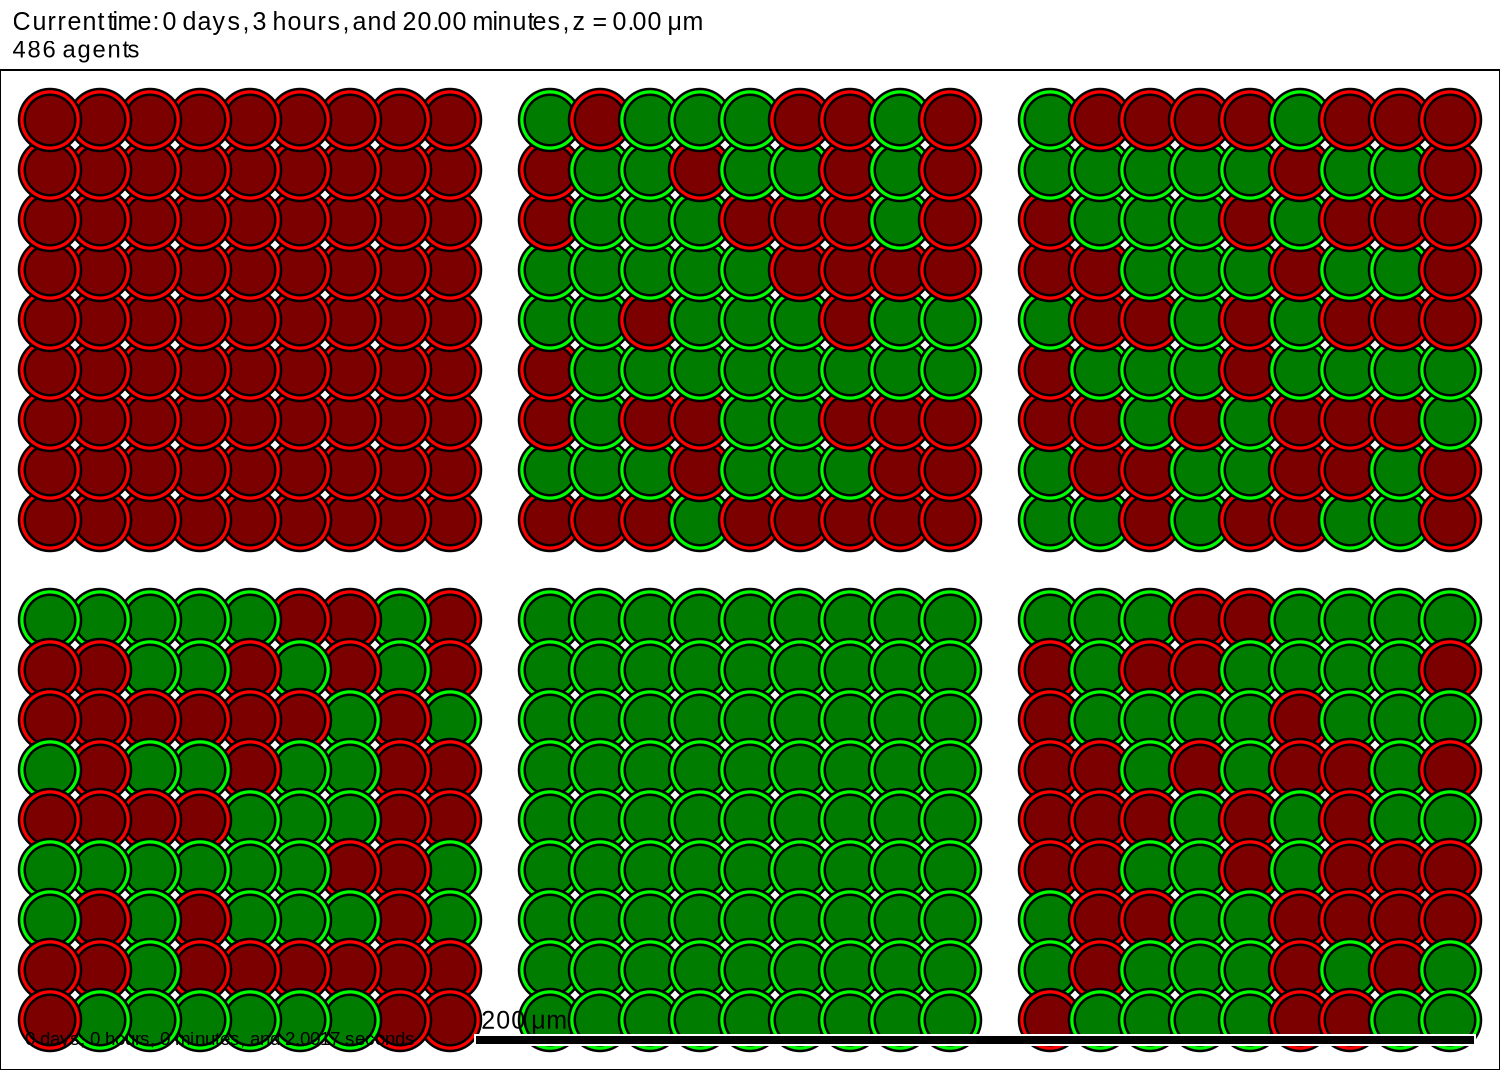
\includegraphics{images/physiboss_cell_lines_example.png}
\end{center}

This population is divided into 6 subpopulations : 

\begin{itemize}
	\item On the bottom left, the cells will need both A and B to be active in order to activate C. Since B is random, around half of the cells will activate B and then C, turning them green.
	
	\item On the bottom middle, we modified the boolean model : cells will need either A or B to activate C. Since A is active in all cells, all of them will activate C and turn green.
	
	\item On the top left, we will mutate the node C to inactive (representing a gene knock-out, for example), so all cells will stay red. We can force any node to be active or inactive to simulate pharmaceutical interventions.
	
	\item On the top middle, we will increase the speed of activation for both B and C : cells will reach steady state faster. Activation and inactivation speed can be controlled by individual parameters, and can also be modified during the simulation.
	
	\item On the bottom right, we will modify this parameter during the simulation : Starting at 0 (B won't activate), the activation speed will set to 0.1 at t=100min. Cells will then start the activation of B and then C.
		
	\item On the top right, we will change the time scale of the whole MaBoSS model : time will go faster, and cells will reach steady state faster. This is particularly useful to combine existing models, where time scales are not necessarily equal (or in the same units).
\end{itemize}

%\TOClink 

% \pagebreak

\section{Future}
\label{sec:Future_Plans}
Several features are planned for upcoming PhysiBoSS releases: 
\begin{enumerate}
\item Simplifying the configuration of the links between PhysiBoSS and PhysiCell, using an automated mapping.

\item Adding new options to define the inheritance of MaBoSS state at cell division. 

\end{enumerate}

\TOClink 

\section{Acknowledgements}
We thank Paul Macklin and Randy Heiland for their help in the creation of this addon. 
\TOClink

\bibliographystyle{abbrvnat}
% \addcontentsline{toc}{chapter}{References}
% \section{References}
\bibliography{references}

\end{document}
